\documentclass[12pt, letterpaper]{article}
\usepackage{amsmath}
\usepackage{tikz}
\usepackage{pgfplots}
\usepackage{enumitem}
\pgfplotsset{compat=1.17}
\usepackage{graphicx} % Required for inserting
\graphicspath{{images/}} %configuring the graphicx package
\newcommand{\iii}{\ensuremath{\int_{a}^{b} f(q)dq}}
\newcommand{\ii}{\ensuremath{\int_{a}^{b}}}

\title{22 Riemann Sums, Evaluating Definite Integrals}
\author{Damiam Alfaro}
\date{January 2 2024}

\begin{document}

\maketitle

\section{First Part: The Definite Integral as Area}
\textbf{Goal}: Compute some definite integrals exactly as areas using geometry.\\
\newline
\textbf{Motivation}: Understand meaningfully how some definite integrals may be computed exactly as areas of some plane regions.\\
\newline
There will be scenarios where you will be given an interval and you will need to approach it using geometry and graph skills. E.g Evaluate:
\[\int_{0}^{4} |6x-5|dx\]
\textbf{a)} write the function as a \(f(x)\) notation so you can solve (or not):
\[f(x)=|6x-5|\]
\textbf{b)} Solve however you can (solve for y, factor, simplify, whatever you can to make it less complex):
\[f(x)=6|x-\frac{5}{6}|\]
\textbf{c)} Graph or imagine the function in a graph so you can reveal the shape within the given interval.
\begin{center}
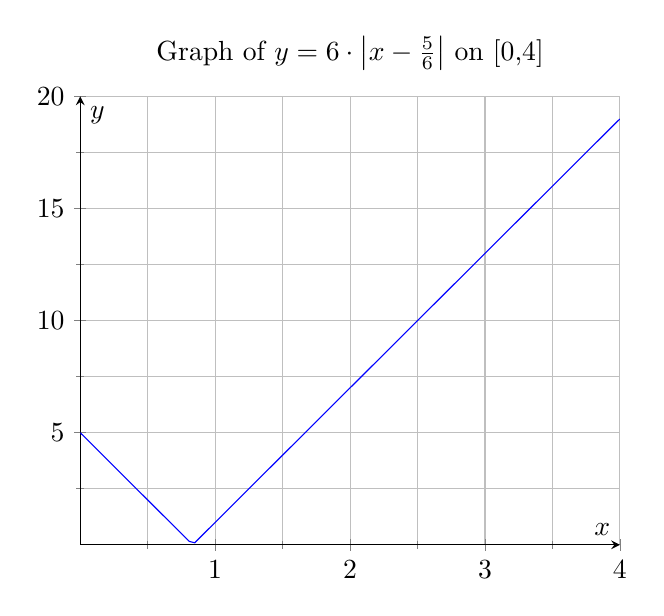
\begin{tikzpicture}
\begin{axis}[
    title={Graph of $y = 6 \cdot \left|x - \frac{5}{6}\right|$ on [0,4]},
    xlabel={$x$},
    ylabel={$y$},
    axis lines=middle,
    ymin=0,
    ymax=20, % Adjusted the maximum y-value to accommodate the function's range
    xmin=0,
    xmax=4, % Set the maximum x-value to 4
    grid=both,
    minor tick num=1
]

% Add the plot for y = 6*|x - 5/6| over the interval [0, 4]
\addplot[blue, samples=100, domain=0:4] {6*abs(x - 5/6)};

\end{axis}
\end{tikzpicture}

\end{center}
\textbf{d)} Identify the geometric figures, and their respective Area formulas: In this case, there are two triangles, one from \([0,\frac{5}{6}]\) and another to \([\frac{5}{6},4]\)
\[A_{triangle} = \frac{1}{2}\cdot b \cdot h\]
\textbf{e)} Perform the areas to the geometric figures, by finding the respective variables within the Area equation: height, lenght, base, etc:
\[A_{t1} = \frac{1}{2}\cdot \left( \frac{5}{6} \right) \cdot (f(0))\]
Before doing the calculations, why the \(f(0)\)? Because that is the point where the vertex happens and the base starts:
\[A_{t1} = \frac{1}{2}\cdot \left( \frac{5}{6} \right) \cdot \left( 6|(0)-\frac{5}{6}| \right)\]
\[A_{t1} = \frac{1}{2}\cdot \left( \frac{5}{6} \right) \cdot (5) = \frac{25}{12}\]
Now Triangle 2
\[A_{t2} = \frac{1}{2}\cdot \left( 4 - \frac{5}{6} \right) \cdot \left( 6|(4)-\frac{5}{6}| \right)\]
Why the \(\left( 4 - \frac{5}{6} \right)\)? Because we are starting to take into account triangle 2 from \(\frac{5}{6}\), and ends in \(4\)
\[A_{t2} = \frac{1}{2}\cdot \left( \frac{19}{6} \right) \cdot \left( 6|\frac{24}{6} - \frac{5}{6}| \right)\]
\[A_{t2} = \frac{361}{12}\]
\textbf{f)} Now in order to solve the integral, add the areas
\[\int_{0}^{4} |6x-5|dx = \frac{361}{12} + \frac{25}{12} = \frac{386}{12} = \frac{193}{6}\]
\section{Second Part: Properties of Definite Integrals}
\textbf{Goal}: Introduce some fundamental properties of definite integrals\\
\newline
\textbf{Motivation}: Understand meaningfully how definite integrals depend on the interval of integration, and how combinations of functions affect them.\\
\newline
Let \(f\) be a piece wise continuous function on \([a,b]\)\\
\newline
\textbf{1)} For any number \(c\) in \([a,b]\)
\[\int_{c}^{c}f(v)dv=0\]
\textbf{2)} Viceversa
\[\int_{a}^{b}f(v)dv=-\int_{b}^{a}f(v)dv\]
\textbf{3)} For any number \(c\) in \([a,b]\)
\[\int_{a}^{c}f(v)dv+\int_{c}^{b}f(v)dv = \int_{a}^{b}f(v)dv\]
\textbf{4) Integral of a constant function}: \(f\) be constant on the interval \([a,b]\), \(f(x)=k\) for all \(x\) in \([a,b]\), then:
\[A = \int_{a}^{b}kdv = k(b-a)\]
This is the area of the rectangle we would be talking about in the example\\
\newline
\textbf{5) Linearity}:
\[\int_{a}^{b}kf(v)dv= k \int_{a}^{b}f(v)dv\]\\
\[\int_{a}^{b}k(f+g)(v)dv= \int_{a}^{b}f(v)dv + \int_{a}^{b}g(v)dv\]
\textbf{6) Comparison}: Let \(f(r) \ge g(r)\) for all \(r\) in \([a,b]\). Then
\[\int_{a}^{b}f(r)dr \ge \int_{a}^{b}g(r)dr\]
\textbf{7) Bounding below and above}: Assume that \(m \ge f(z) \ge M\) for all \(z\) in \([a,b]\), then:
\[m(b-a) \le \ii \le M(b-a)\]
\textbf{8) Integral of zero (null) function}: Assume that \(f(t)=0\) for all \(t\) in \([a,b]\). Then:
\[\ii = 0\]
\textbf{9) Integral of a difference of two functions}:
\[\int_{a}^{b}(f-g)(q)dq = \iii - \int_{a}^{b}g(r)dr\]
\textbf{10) Integral of a linear combination of functions} (let k and l be constants)
\[\int_{a}^{b} (kf+lg)(p)dp = k\ii f(s)ds + l\ii g(t)dt\]




\end{document}
